\documentclass[]{article}

\usepackage{graphicx}

%opening
\title{Figures for  3-D printed oxygen devices}
\author{}

\begin{document}

%\maketitle

\section{figures}

\begin{figure}[H]
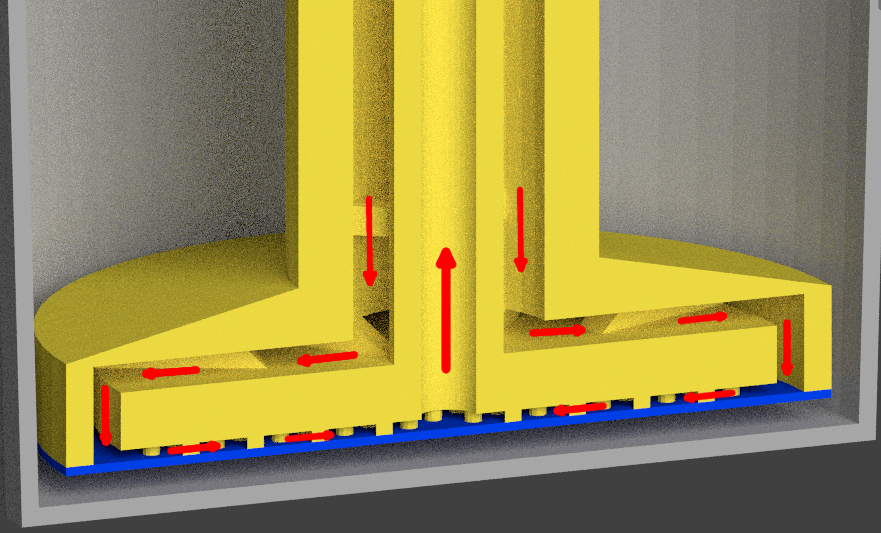
\includegraphics[scale=0.2]{../presentation-figures/piller-well-render-with-arrows.png} % remove for manuscript submission
\caption{
{\bf CAD rendering of the piller bottom.} The 'Pipe with in a pipe' flow pattern delivers gas to the bottom of each well where it diffuses to the culture.  
}
\label{piller-well-render-figure}
\end{figure}

\begin{figure}[H]
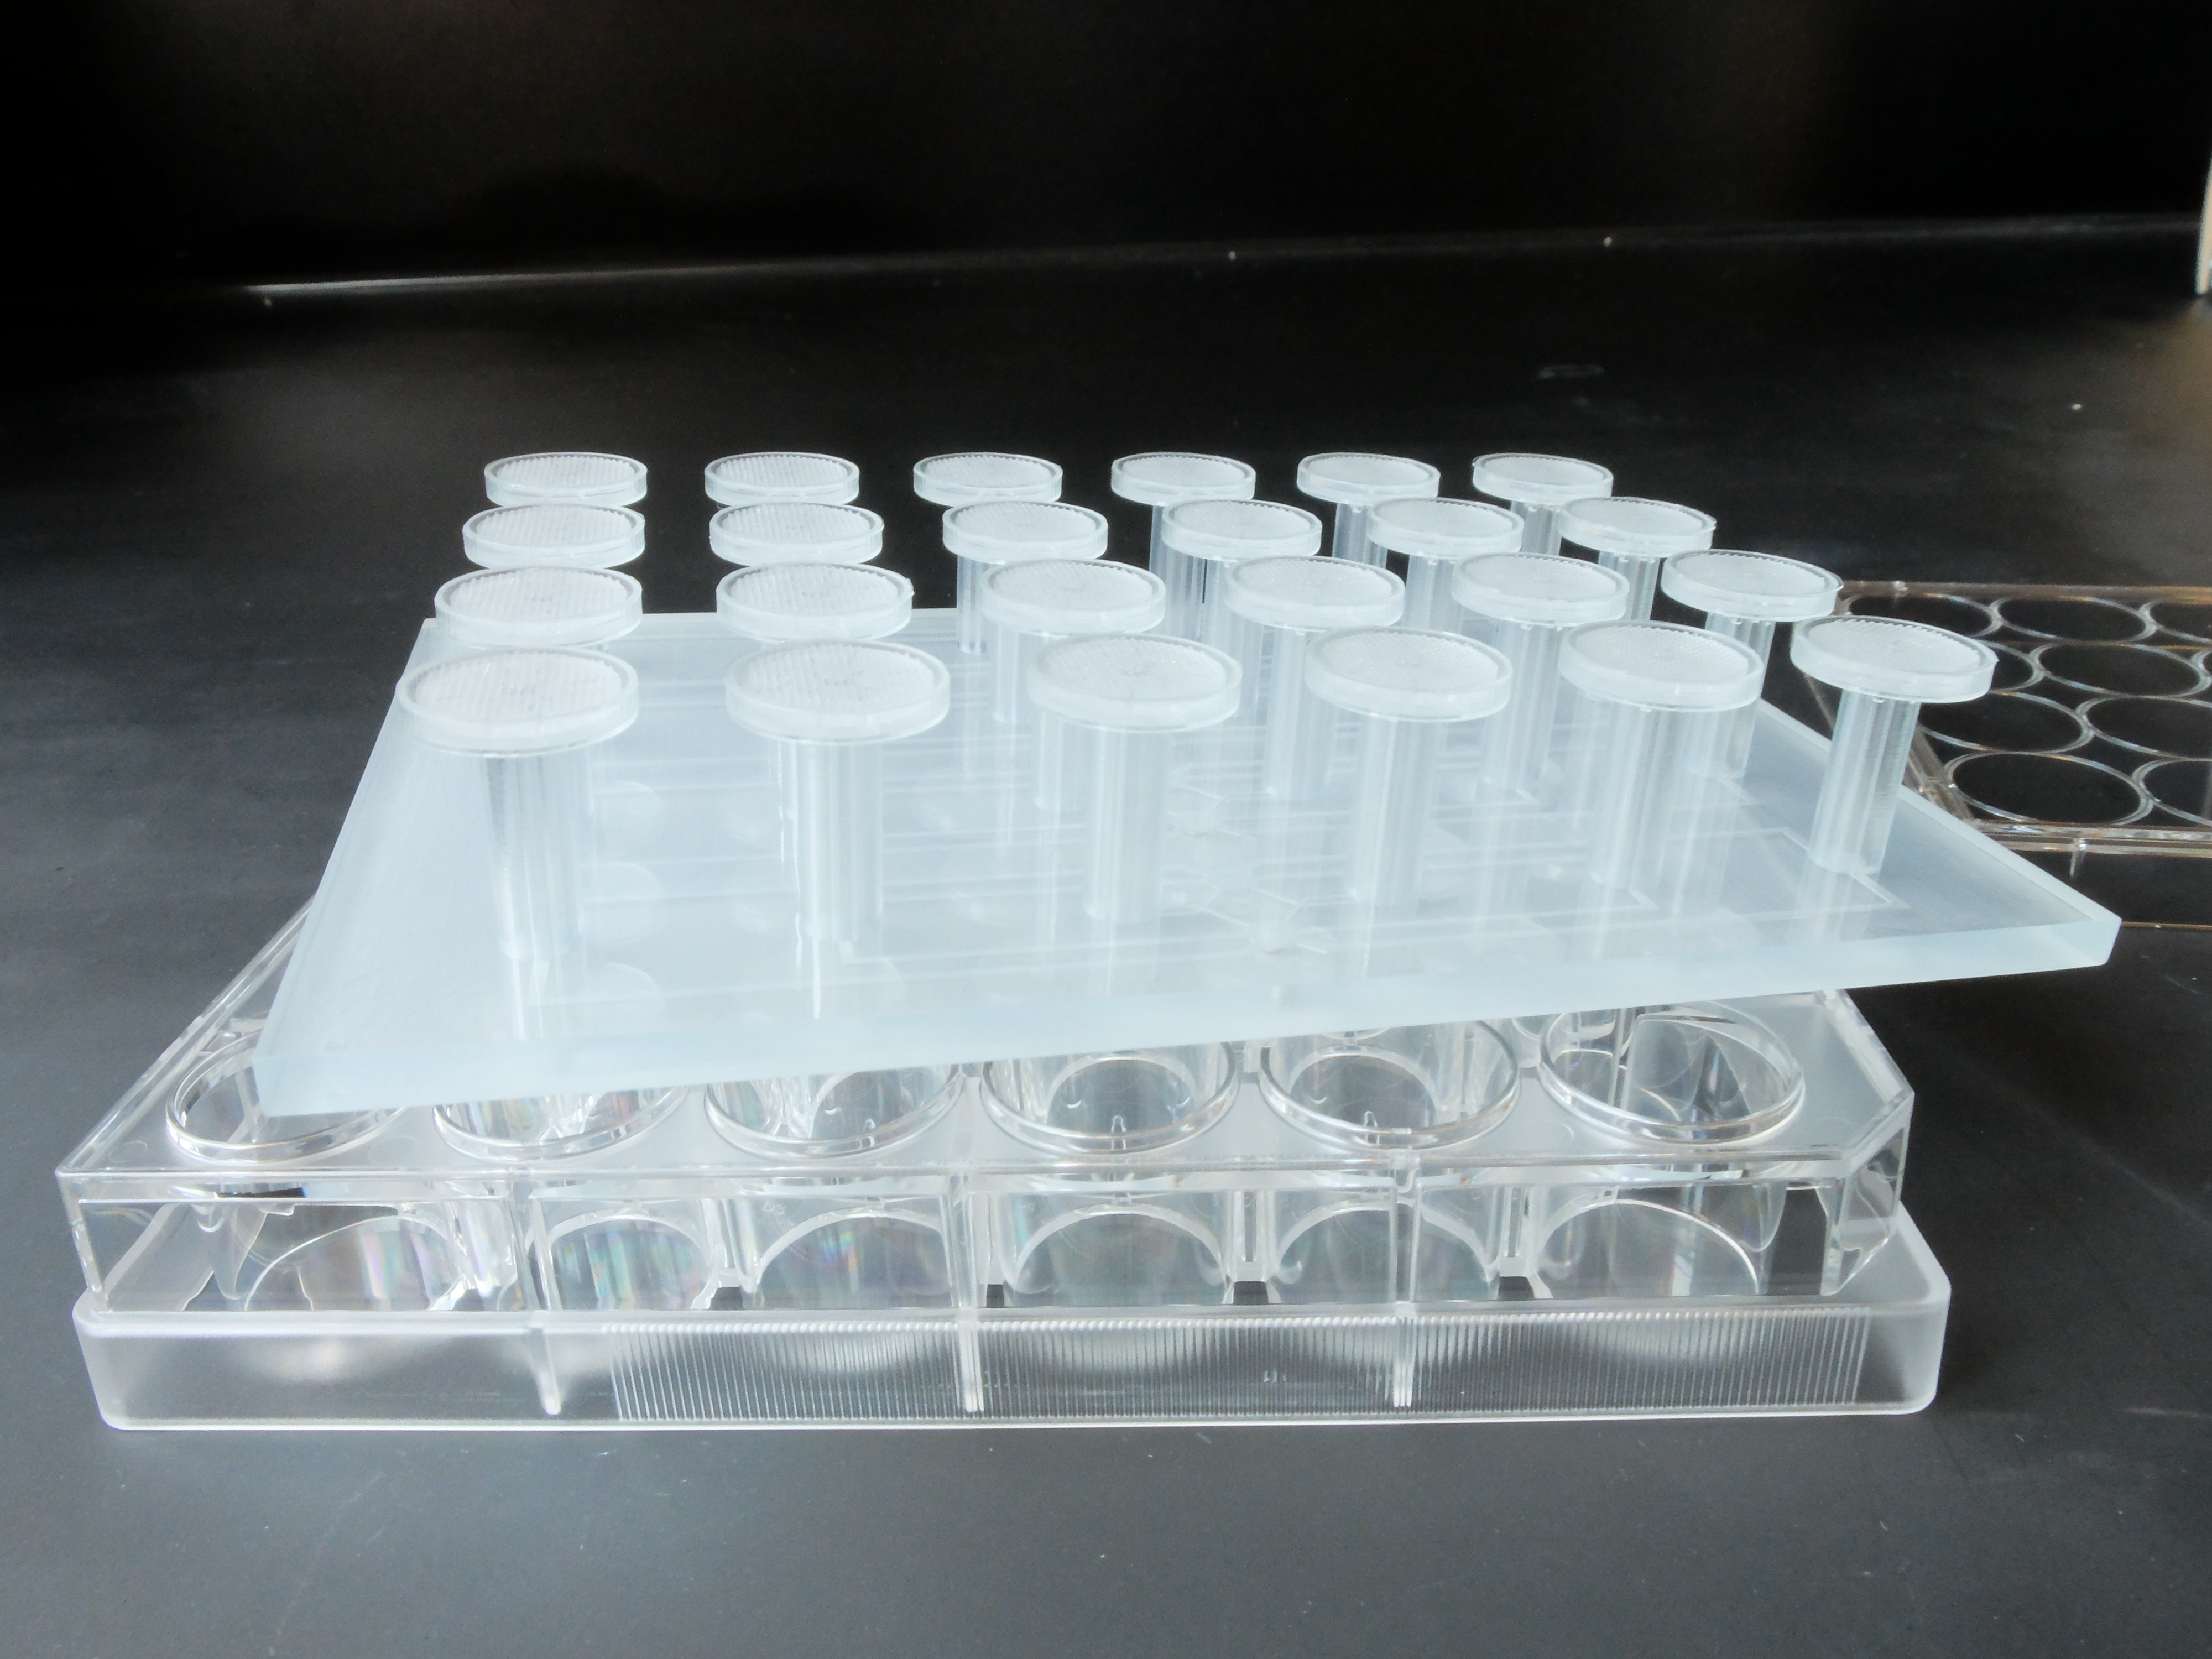
\includegraphics[scale=0.05]{../presentation-figures/24well.JPG} % remove for manuscript submission
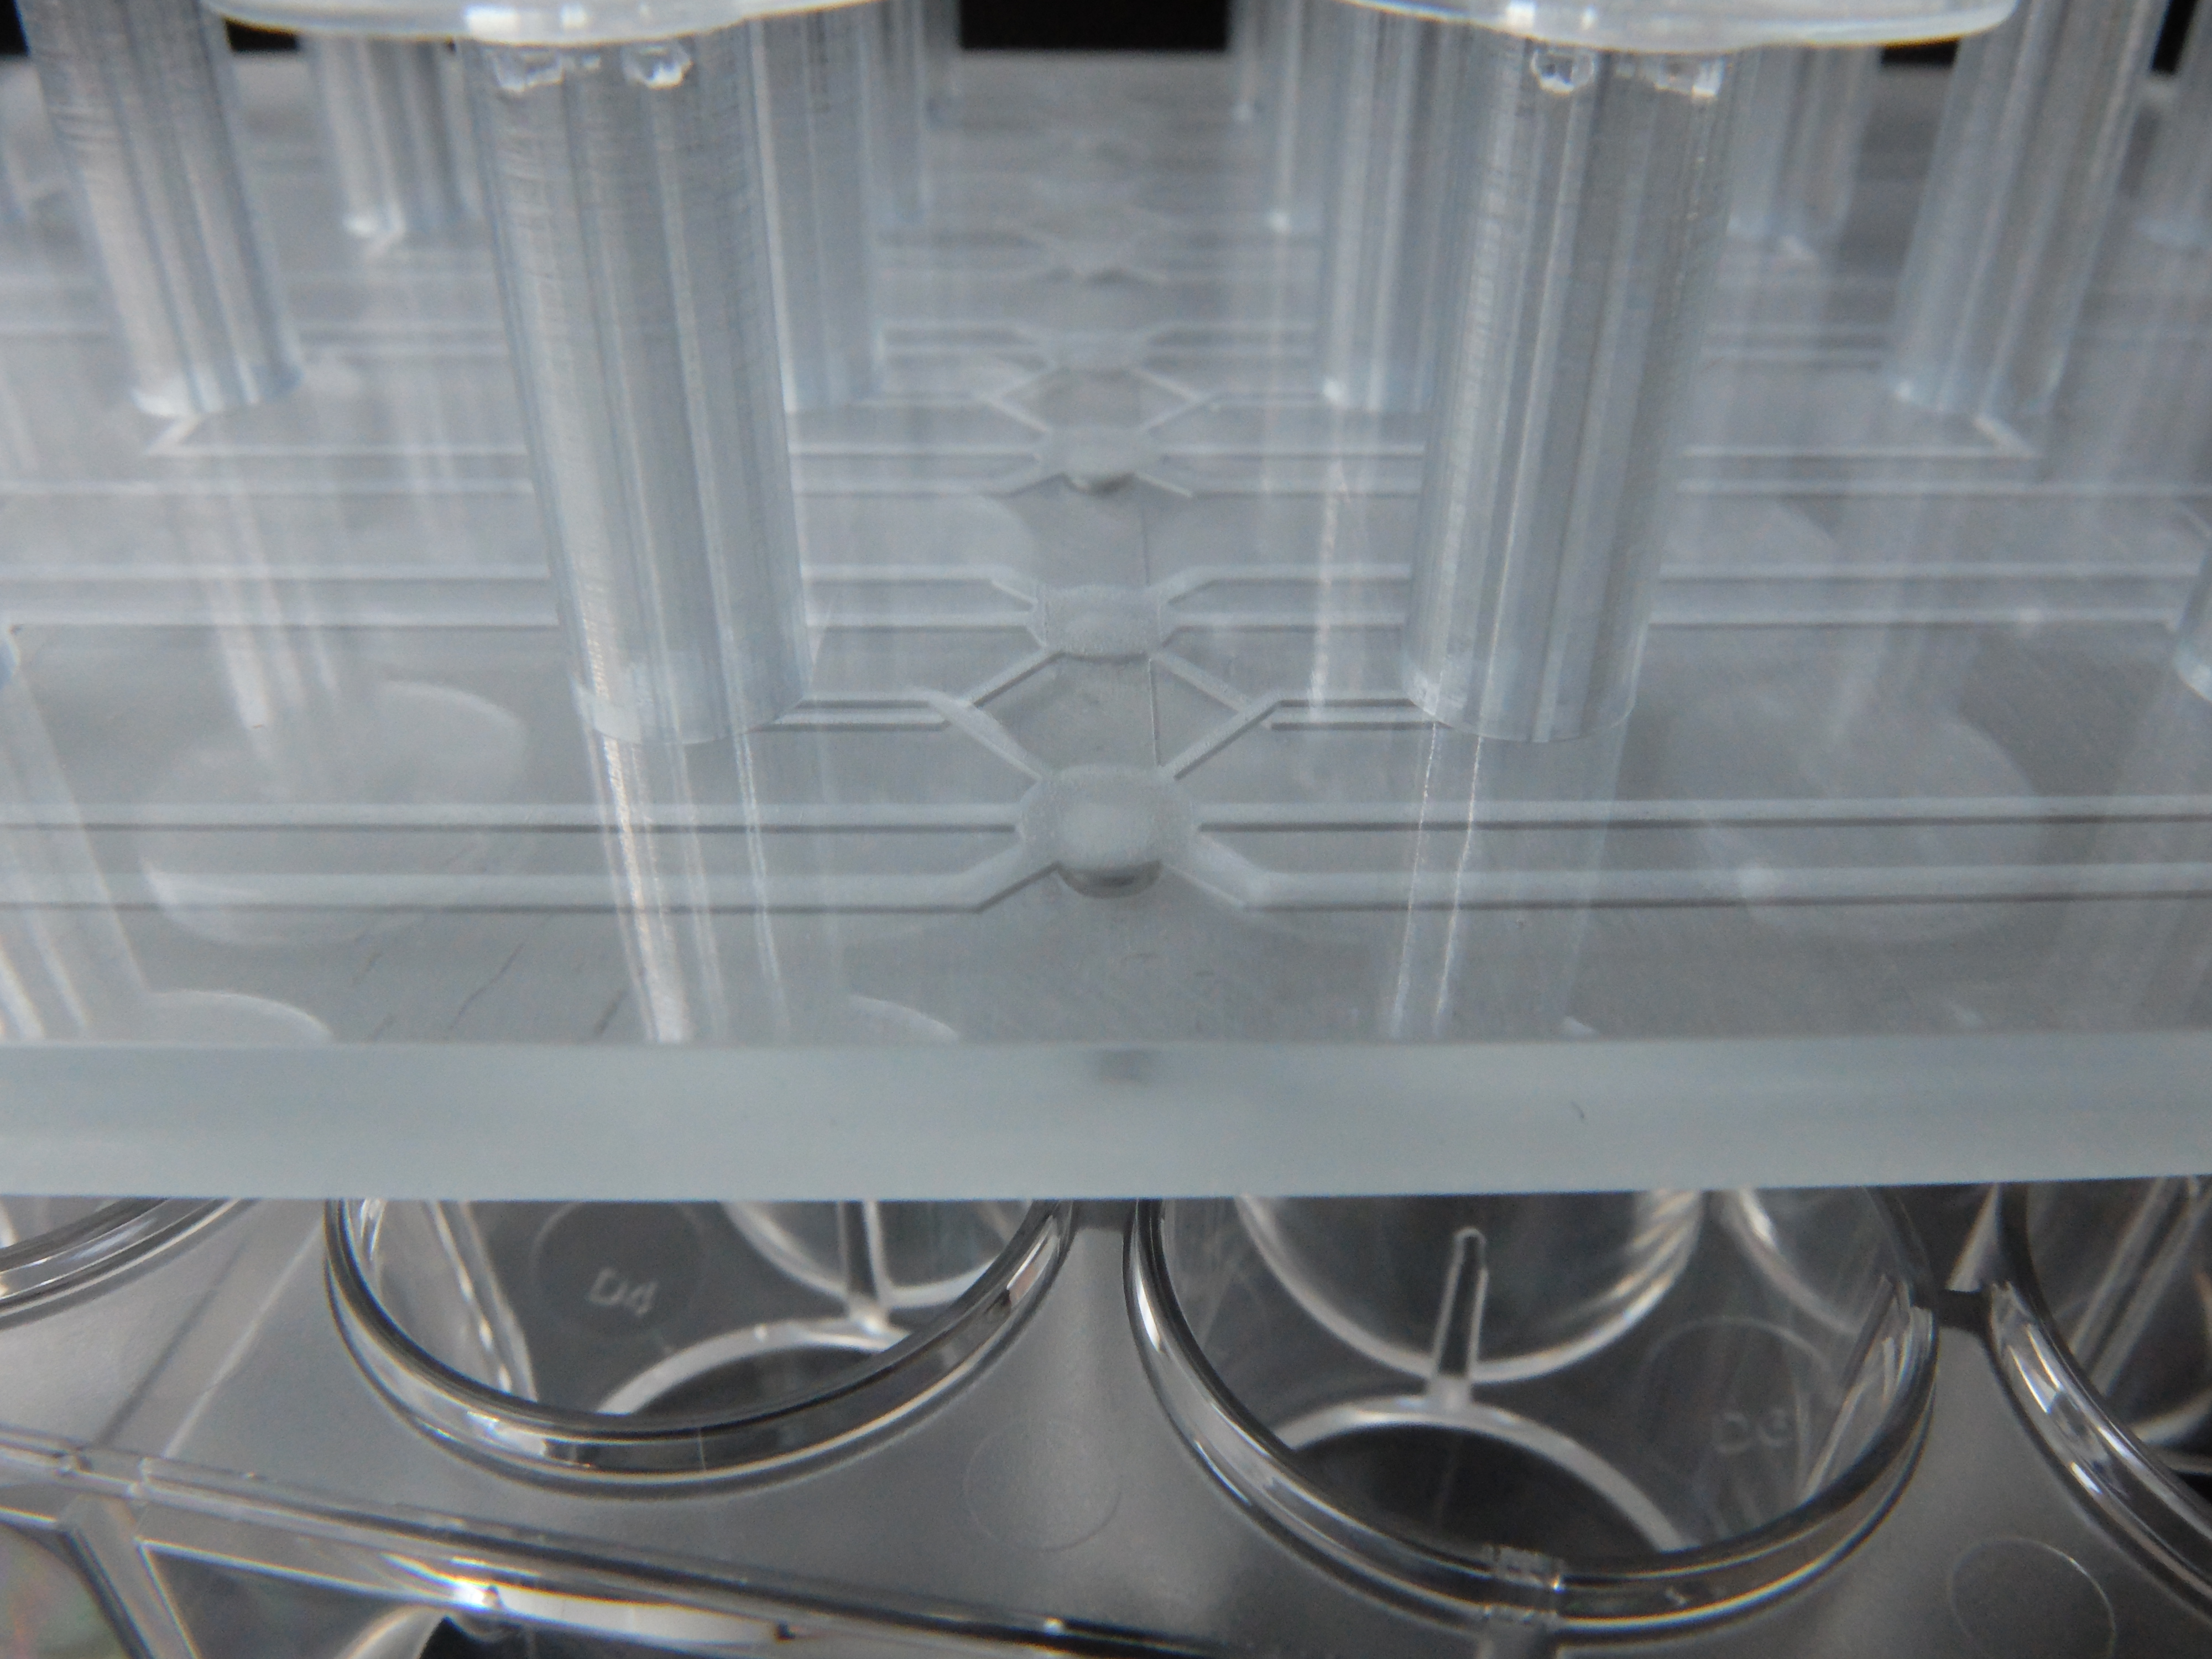
\includegraphics[scale=0.05]{../presentation-figures/printed-network.JPG} % remove for manuscript submission
\caption{
{\bf Photographs of the printed device.}  The printed device with membranes adhered. The distribution network is printed completely in resin.
}
\label{device-photos-figure}
\end{figure}

\begin{figure}[H]
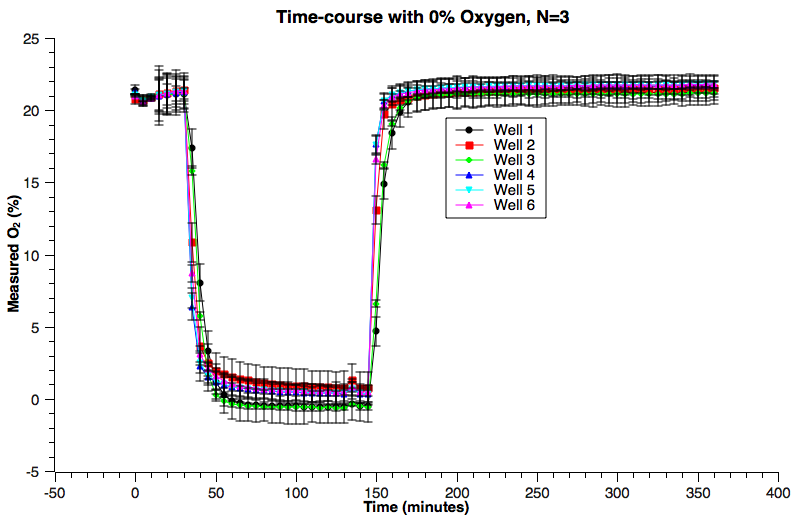
\includegraphics[scale=0.3]{../presentation-figures/6-well-plot.png} % remove for manuscript submission
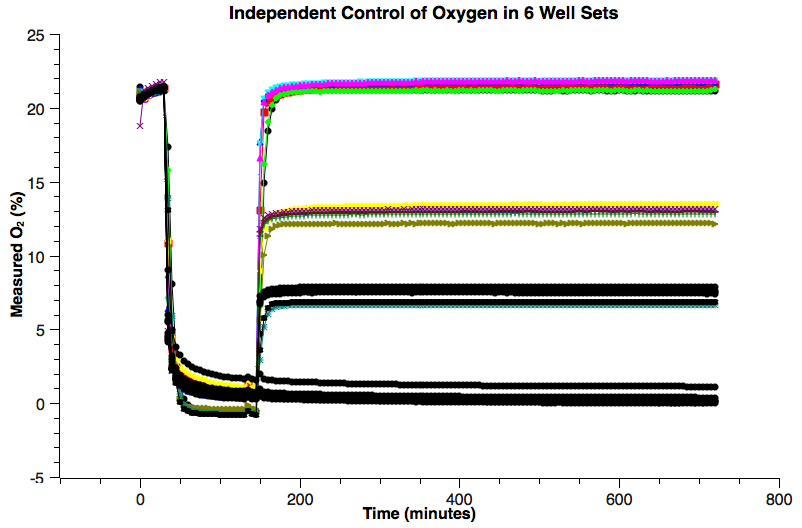
\includegraphics[scale=0.3]{../presentation-figures/24-well-plot.png} % remove for manuscript submission
\caption{
{\bf Oxygen Characterization.}  Time course data of oxygen being evacuated from the culture area as 0\% oxygen gas is perfused through the device. Each 6 well row of the plate can be controlled independently.  
}
\label{oxygen-char-figure}
\end{figure}

\begin{figure}[H]
%\includegraphics[scale=0.2]{image.jpg} % remove for manuscript submission
\caption{
{\bf PCR Data.}  Not finished yet.  
}
\label{pcr-data}
\end{figure}

%\begin{abstract}

%\end{abstract}

%\section{}

\end{document}
